\documentclass[tikz,border=2pt]{standalone}
\usepackage{amsmath,amssymb}
\usepackage{tikz}
\usetikzlibrary{matrix}

\begin{document}
% The main diagonal runs from the top-left corner down to the right: the entries a_ii.
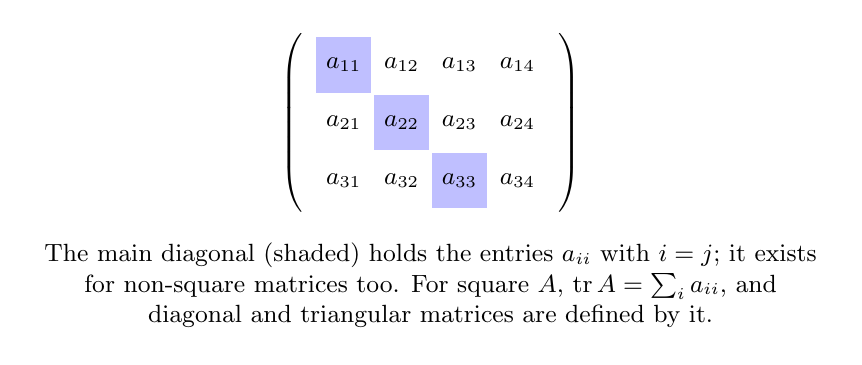
\begin{tikzpicture}[every node/.style={font=\small}]
	\matrix (A) [matrix of math nodes, nodes={minimum size=7mm, anchor=center}, left delimiter=(, right delimiter=), column sep=1pt, row sep=1pt] at (0,0) {
		|[fill=blue!25]| a_{11} & a_{12} & a_{13} & a_{14} \\
		a_{21} & |[fill=blue!25]| a_{22} & a_{23} & a_{24} \\
		a_{31} & a_{32} & |[fill=blue!25]| a_{33} & a_{34} \\
	};
	\node[anchor=north, align=flush center, text width=10cm] at (0,-1.4) {The main diagonal (shaded) holds the entries $a_{ii}$ with $i=j$; it exists for non-square matrices too. For square $A$, $\operatorname{tr}A=\sum_i a_{ii}$, and diagonal and triangular matrices are defined by it.};
\end{tikzpicture}
\end{document}
